\documentclass[10pt,dvipsnames]{beamer}
\usepackage[T1]{fontenc}
\usepackage{libertinus}
\usepackage{amsmath}
\usepackage[most]{tcolorbox}
\usepackage{graphicx}

\usepackage{hyperref}
%python 
\usepackage{listings}
% Default fixed font does not support bold face
\DeclareFixedFont{\ttb}{T1}{txtt}{bx}{n}{8} % for bold
\DeclareFixedFont{\ttm}{T1}{txtt}{m}{n}{8}  % for normal

% Custom colors
\usepackage{color}
\definecolor{deepblue}{rgb}{0,0,0.5}
\definecolor{deepred}{rgb}{0.6,0,0}
\definecolor{deepgreen}{rgb}{0,0.5,0}

\usepackage{listings}

% Python style for highlighting
\newcommand\pythonstyle{\lstset{
		language=Python,
		basicstyle=\ttm,
		morekeywords={self},              % Add keywords here
		keywordstyle=\ttb\color{deepblue},
		emph={MyClass,__init__},          % Custom highlighting
		emphstyle=\ttb\color{deepred},    % Custom highlighting style
		stringstyle=\color{deepgreen},
		frame=tb,                         % Any extra options here
		showstringspaces=false
}}


% Python environment
\lstnewenvironment{python}[1][]
{
	\pythonstyle
	\lstset{#1}
}
{}

% Python for external files
\newcommand\pythonexternal[2][]{{
		\pythonstyle
		\lstinputlisting[#1]{#2}}}

% Python for inline
\newcommand\pythoninline[1]{{\pythonstyle\lstinline!#1!}}

\usepackage{xcolor}  
\newcommand{\cb}[1]{{\color{CadetBlue}#1}}

\usepackage{pgfplots}
\pgfplotsset{compat=newest}
\setlength{\parskip}{0.5em}

\usepackage{setspace}
\setstretch{1.25}  
\usetheme{Singapore}
\setbeamertemplate{navigation symbols}{}


\title{CSE574 Introduction to Machine Learning}
\subtitle{Discriminant Analysis}
\author{Jue Guo}
\institute{University at Buffalo}
\date{\today}

\begin{document}
\begin{frame}
	\titlepage
\end{frame}
\begin{frame}
	\frametitle{Outline}
	\tableofcontents
\end{frame}

\section{Learning Objective}
\begin{frame}{Learning Objective}
	\begin{itemize}
		\item Define discriminant function and linear discriminant analysis.
		\item Use discriminant functions to classify an instance.
		\item Define covariance.
		\item Use covariance and class means to calculate linear discriminant weights.
		\item Define principal components.
		\item Explain when the principal components technique is useful.
	\end{itemize}
\end{frame}

\section{Linear Discriminant Analysis}
\begin{frame}{Linear Discriminant Analysis}
	A \textbf{discriminant function}, denoted \(\delta(\mathbf{x})\), is a function used to set a decision boundary between classes.
	\begin{itemize}
		\item Each class has a unique discriminant function, \(\delta_{i}(\mathbf{x})\), and the class with the highest discriminant function for a given set of input values is the predicted class.
		\item Ex: In logistic regression, the probabilities of class 1 vs. class 0 are discriminant functions \(-\delta_{1}(\mathbf{x})=\hat{p}_{i}=\frac{\exp \left(w_{0}+w_{1} x_{i}\right)}{1+\exp \left(w_{0}+w_{1} x_{i}\right)}\) vs.
		      \(\delta_{0}(\mathbf{x})=1-\frac{\exp \left(w_{0}+w_{1} x_{i}\right)}{1+\exp \left(w_{0}+w_{1} x_{i}\right)}\).
	\end{itemize}
	If \(\delta_{1}(\mathbf{x}) \geq \delta_{0}(\mathbf{x})\), then the instance is predicted as class 1 .
\end{frame}

\begin{frame}{Linear Discriminant Analysis}
	\textbf{Linear discriminant analysis} classifies instances by comparing linear discriminant functions.
	\begin{itemize}
		\item Each discriminant function in linear discriminant analysis estimates the natural log of the conditional probability of class \(i_{1} P\left(y_{i} \mid \mathbf{x}\right)\), based on a linear function of the input features.
	\end{itemize}
	$$
		\delta_{i}(\mathbf{x})=\ln \left(P\left(y_{i} \mid \mathbf{x}\right)\right)=\mathbf{w}_{i}^{T} \mathbf{x}+w_{i 0}
	$$
	where \(\mathbf{w}\) is a vector of weights for each input feature on class \(i\), and \(w_{i 0}\) is an intercept term for class \(i\).
	The class with the highest discriminant function, \(\delta_{i}(\mathbf{x})=\ln \left(P\left(y_{i} \mid \mathbf{x}\right)\right)\), is the predicted class.
	\begin{itemize}
		\item 	The linear discriminant weights \(\mathbf{w}\) are chosen so that the discriminant functions capture as much variation in the input features as possible while accurately classifying instances.
	\end{itemize}
\end{frame}

\begin{frame}{Classification using linear discriminant functions}
	\begin{figure}[ht]
		\centering
		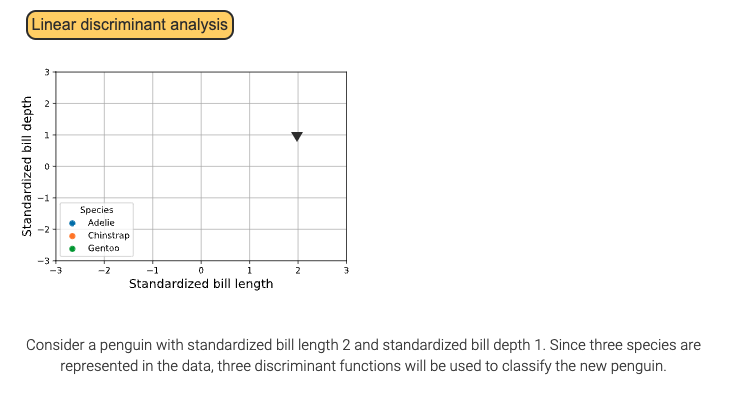
\includegraphics[width=\textwidth]{imgs/df_1.png}
	\end{figure}
\end{frame}

\begin{frame}{Classification using linear discriminant functions}
	\begin{figure}[ht]
		\centering
		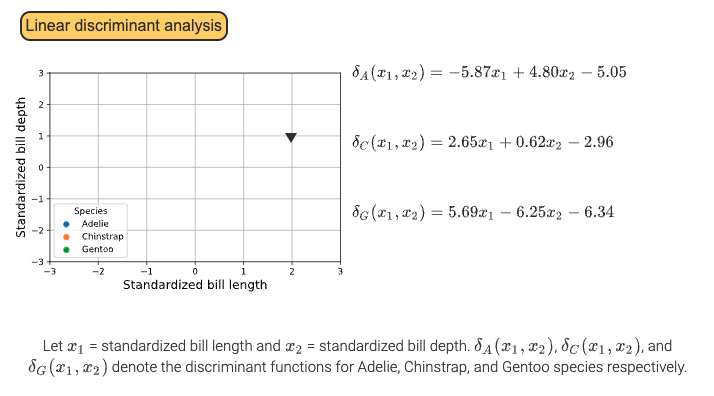
\includegraphics[width=\textwidth]{imgs/df_2.png}
	\end{figure}
\end{frame}

\begin{frame}{Classification using linear discriminant functions}
	\begin{figure}[ht]
		\centering
		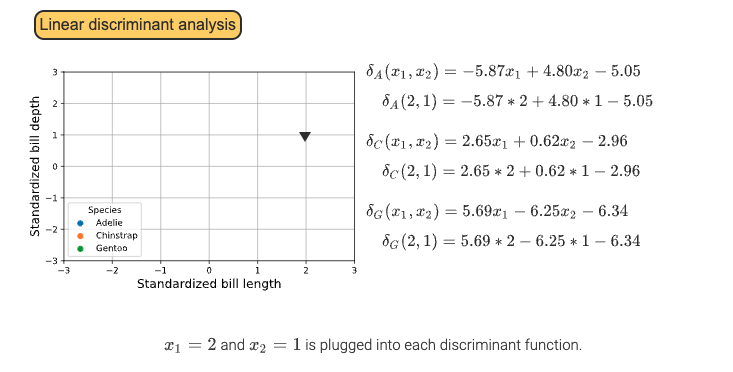
\includegraphics[width=\textwidth]{imgs/df_3.png}
	\end{figure}
\end{frame}

\begin{frame}{Classification using linear discriminant functions}
	\begin{figure}[ht]
		\centering
		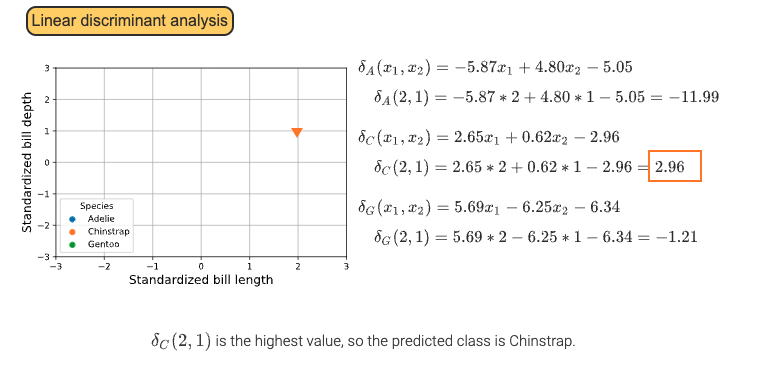
\includegraphics[width=\textwidth]{imgs/df_4.png}
	\end{figure}
\end{frame}

\section{Calculating Discriminant Weights using Covariance}
\begin{frame}{Calculating Discriminant Weights using Covariance}
	Let \(\mathbf{w}_{i}\) be the discriminant function weights for class \(i\). The discriminant weights for standardized input features are calculated using two quantities:
	\begin{itemize}
		\item Class means for feature \(i\), denoted \(\mu_{\mathbf{i}}\).
		\item Covariance matrix, denoted \(\boldsymbol{\Sigma}\).
	\end{itemize}
\end{frame}

\begin{frame}{Calculating Discriminant Weights using Covariance}
	\begin{itemize}
		\item \textbf{Covariance} measures how values of one feature change in relation to a second feature, denoted \(\sigma_{i j}^{2}\). Features with \(\sigma_{i j}^{2}=0\) are uncorrelated, or independent. The variance between feature \(i\) and itself is the variance \(\sigma_{i}^{2}\).
		\item  A \textbf{covariance matrix} is a matrix containing all pairwise covariances between features \(i\) and \(j\), denoted \(\Sigma\).
		      $$
			      \boldsymbol{\Sigma}=\left[\begin{array}{cccc}\sigma_{1}^{2} & \sigma_{12}^{2} & \ldots & \sigma_{1 p}^{2} \\ \sigma_{12}^{2} & \sigma_{2}^{2} & \ldots & \sigma_{2 p}^{2} \\ \vdots & \vdots & \ddots & \vdots \\ \sigma_{1 p}^{2} & \sigma_{2 p}^{2} & \ldots & \sigma_{p}^{2}\end{array}\right]
		      $$
	\end{itemize}
\end{frame}

\begin{frame}{Calculating Discriminant Weights using Covariance}
	The discriminant function weights in linear discriminant analysis are
	$$
		\mathbf{w}_{i}=\boldsymbol{\Sigma}^{-1} \mu_{i}
	$$
	$$
		w_{0 i}=-\frac{1}{2} \mu_{i}^{T} \mathbf{w}_{i}+\ln (P(y=i))
	$$
	where \(\boldsymbol{\Sigma}^{-1}\) is the inverse of the covariance matrix and \(P(y=i)\) is the prior probability of class \(i\).

	\begin{itemize}
		\item The discriminant weights \(w_{i}\) are a weighted function of the class means.
		\item The intercept \(w_{0 i}\) is a weighted function of the discriminant weights plus the natural log of the prior probability for class \(i, P(y=i)\).
		\item The prior probability \(P(y=i)\) may be estimated from the data or based on external assumptions.
	\end{itemize}
\end{frame}

\begin{frame}{Calculating discriminant weights for Adelie penguins.}
	\begin{figure}[ht]
		\centering
		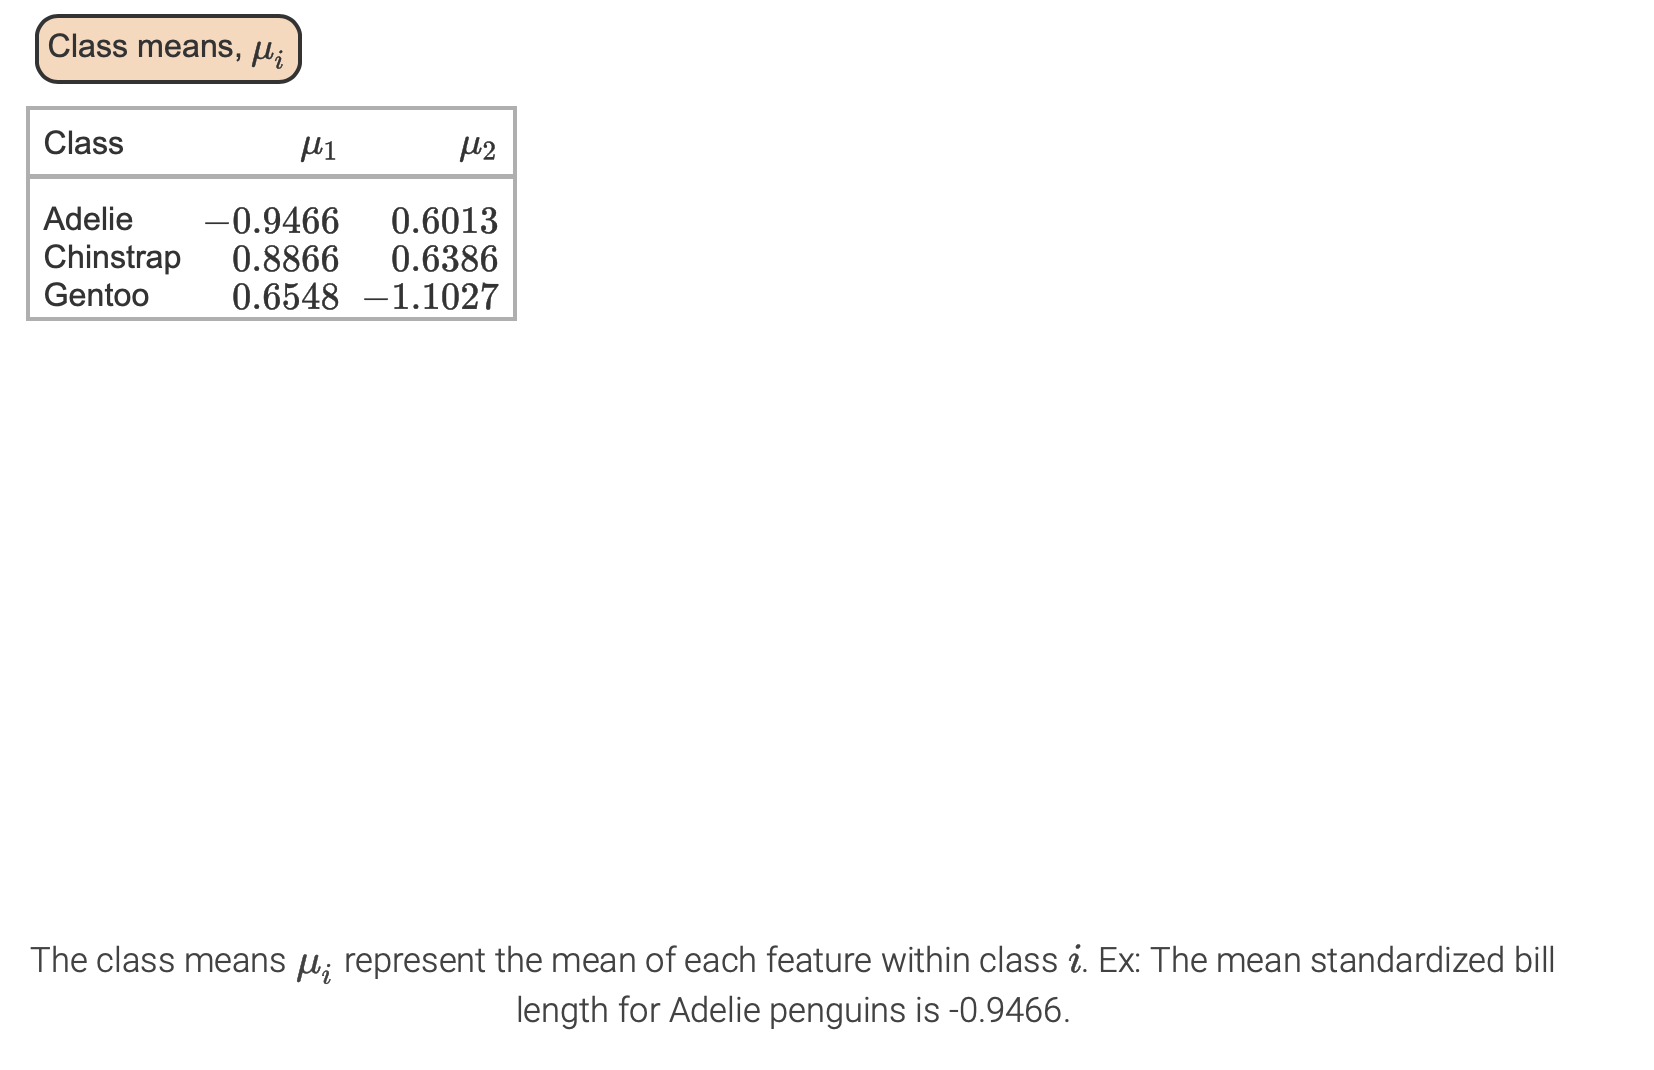
\includegraphics[width=0.8\textwidth]{imgs/df_5.png}
	\end{figure}
\end{frame}

\begin{frame}{Calculating discriminant weights for Adelie penguins.}
	\begin{figure}[ht]
		\centering
		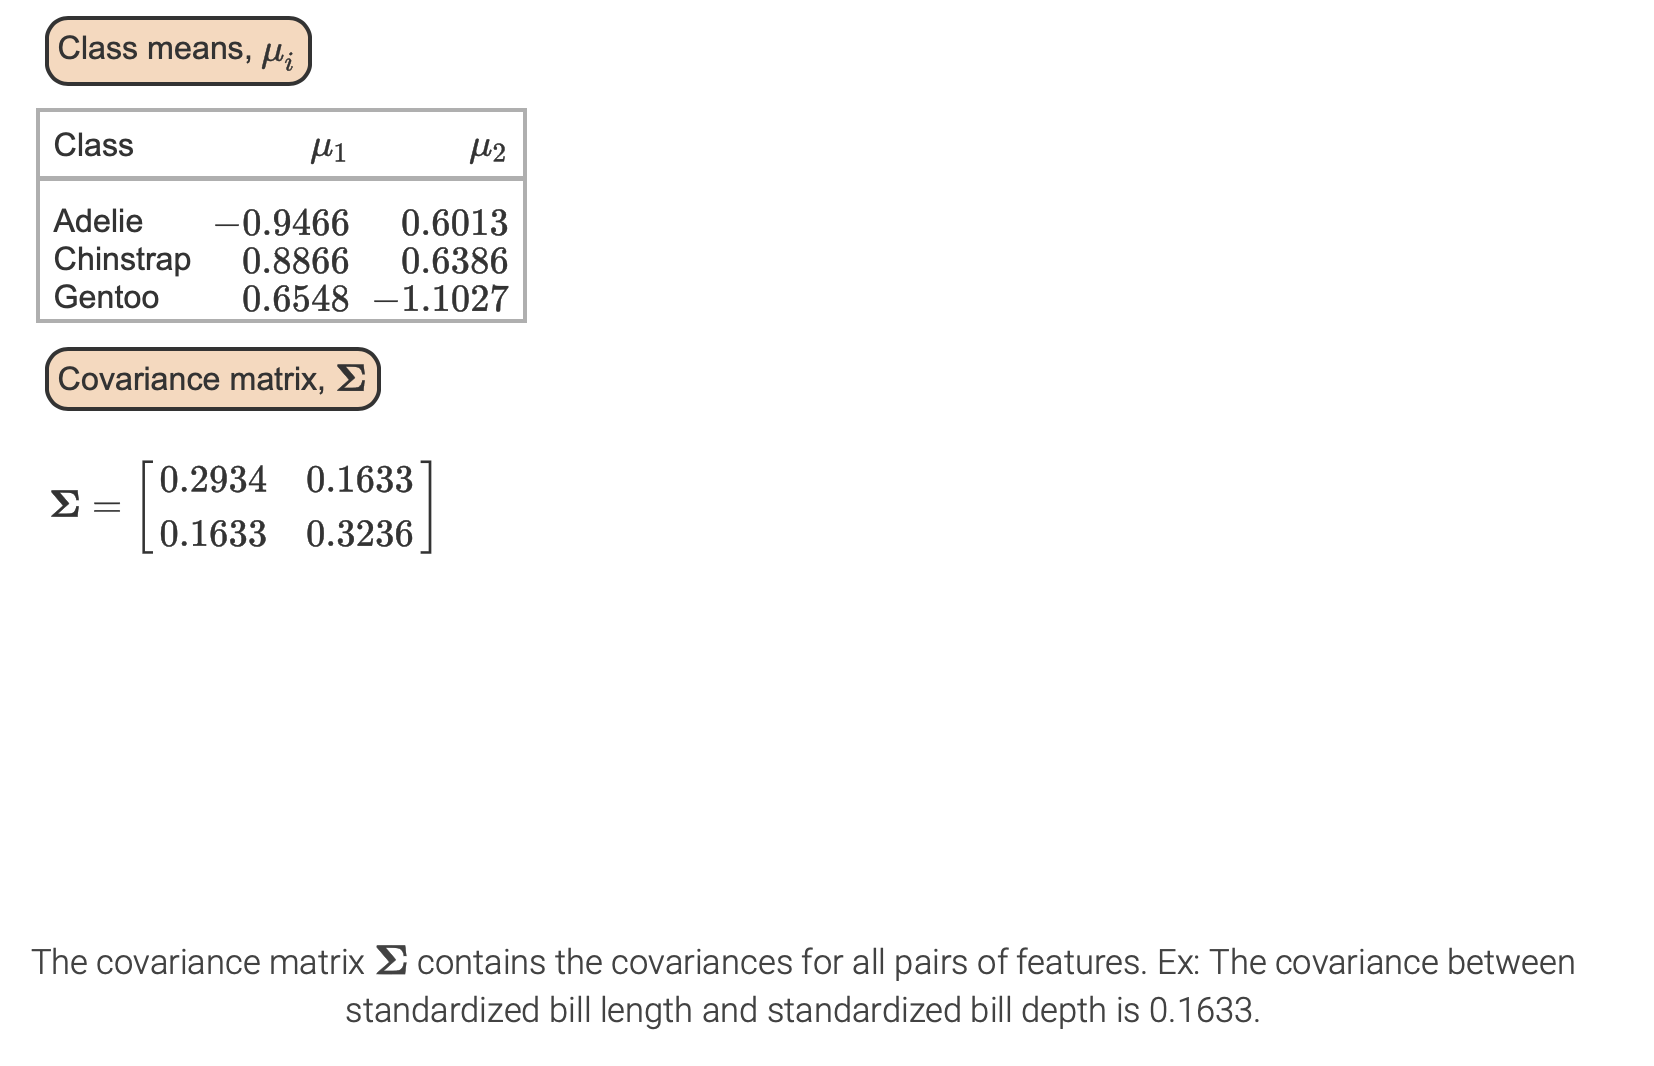
\includegraphics[width=0.8\textwidth]{imgs/df_6.png}
	\end{figure}
\end{frame}

\begin{frame}{Calculating discriminant weights for Adelie penguins.}
	\begin{figure}[ht]
		\centering
		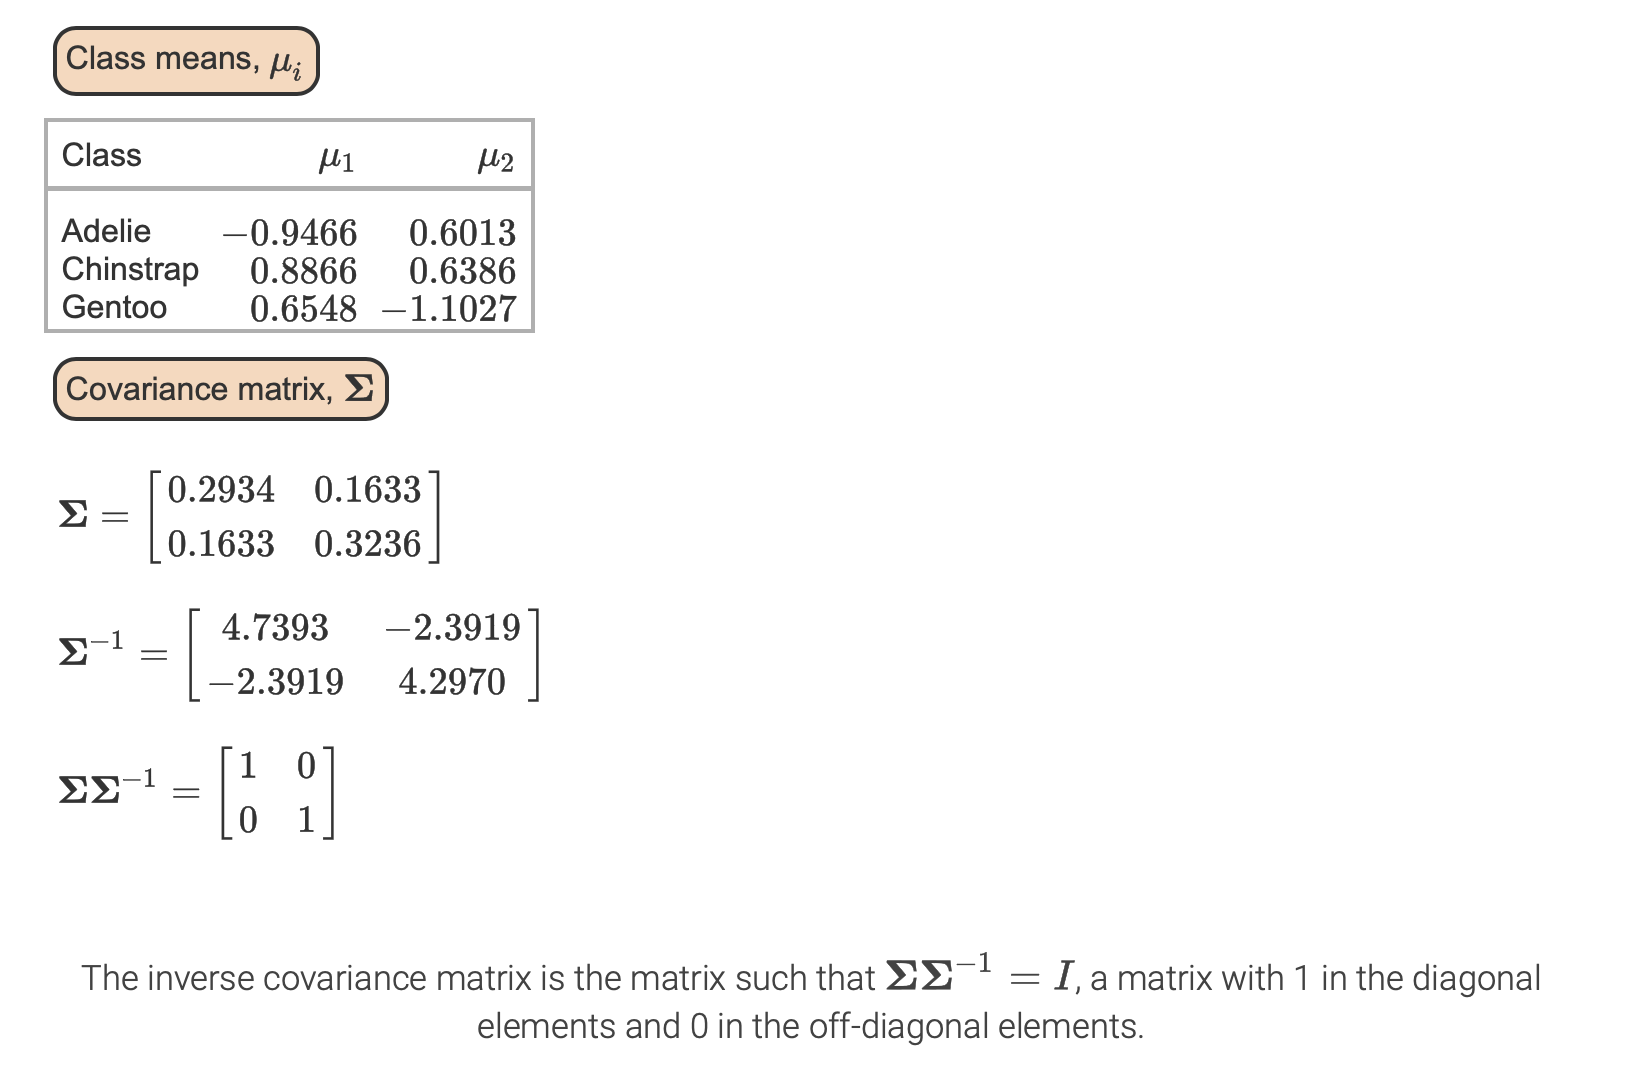
\includegraphics[width=0.8\textwidth]{imgs/df_7.png}
	\end{figure}
\end{frame}

\begin{frame}{Calculating discriminant weights for Adelie penguins.}
	\begin{figure}[ht]
		\centering
		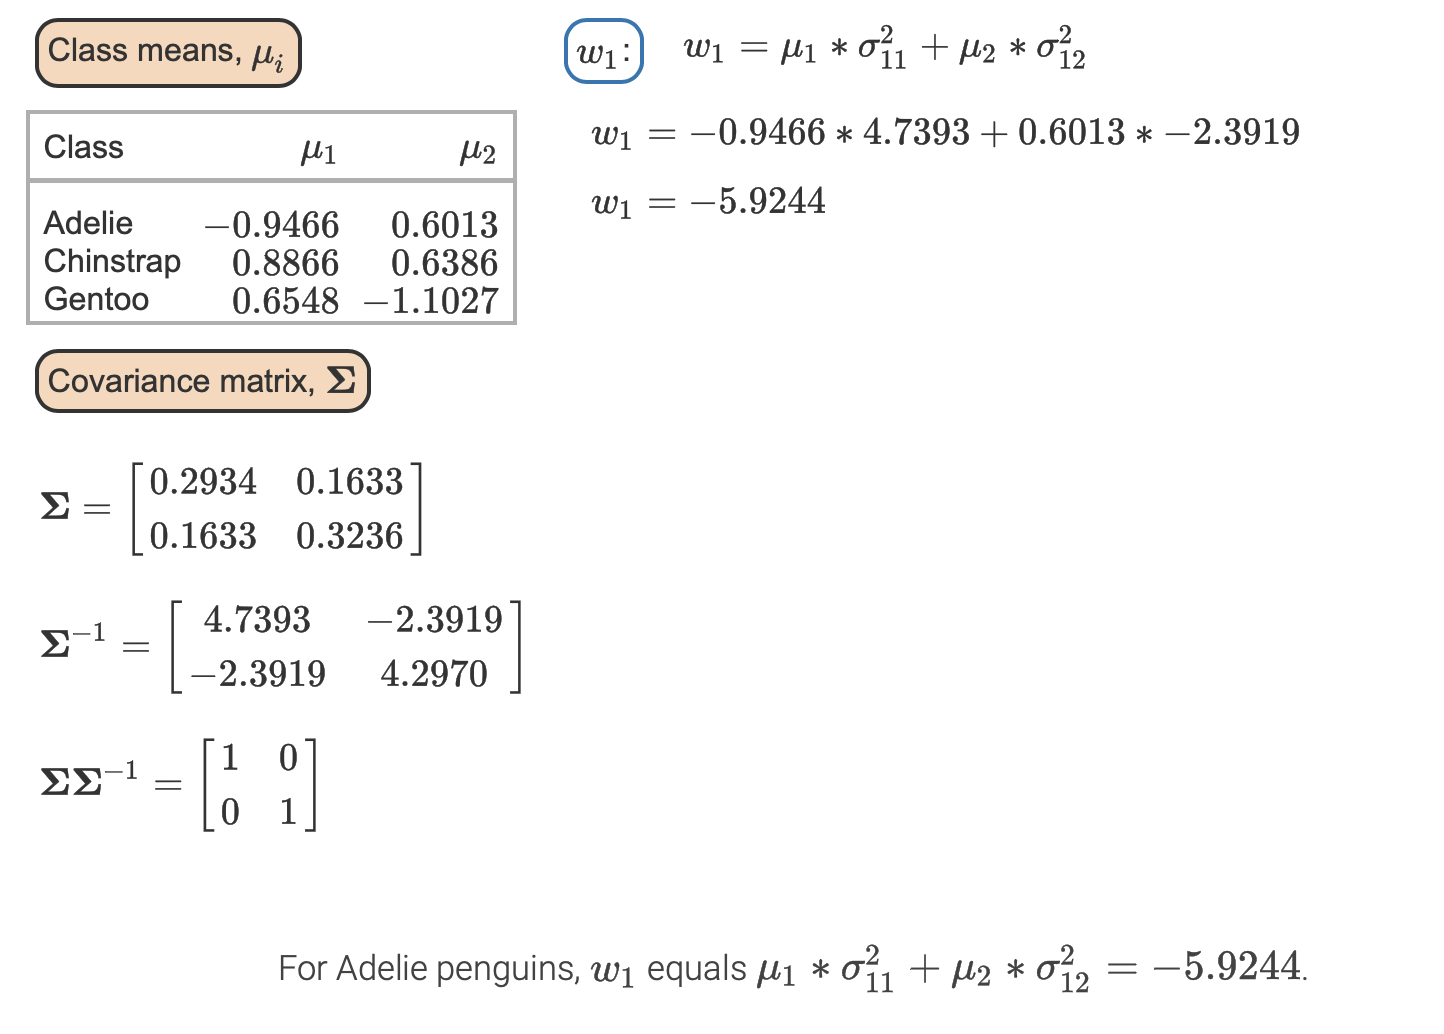
\includegraphics[width=0.8\textwidth]{imgs/df_8.png}
	\end{figure}
\end{frame}

\begin{frame}{Calculating discriminant weights for Adelie penguins.}
	\begin{figure}[ht]
		\centering
		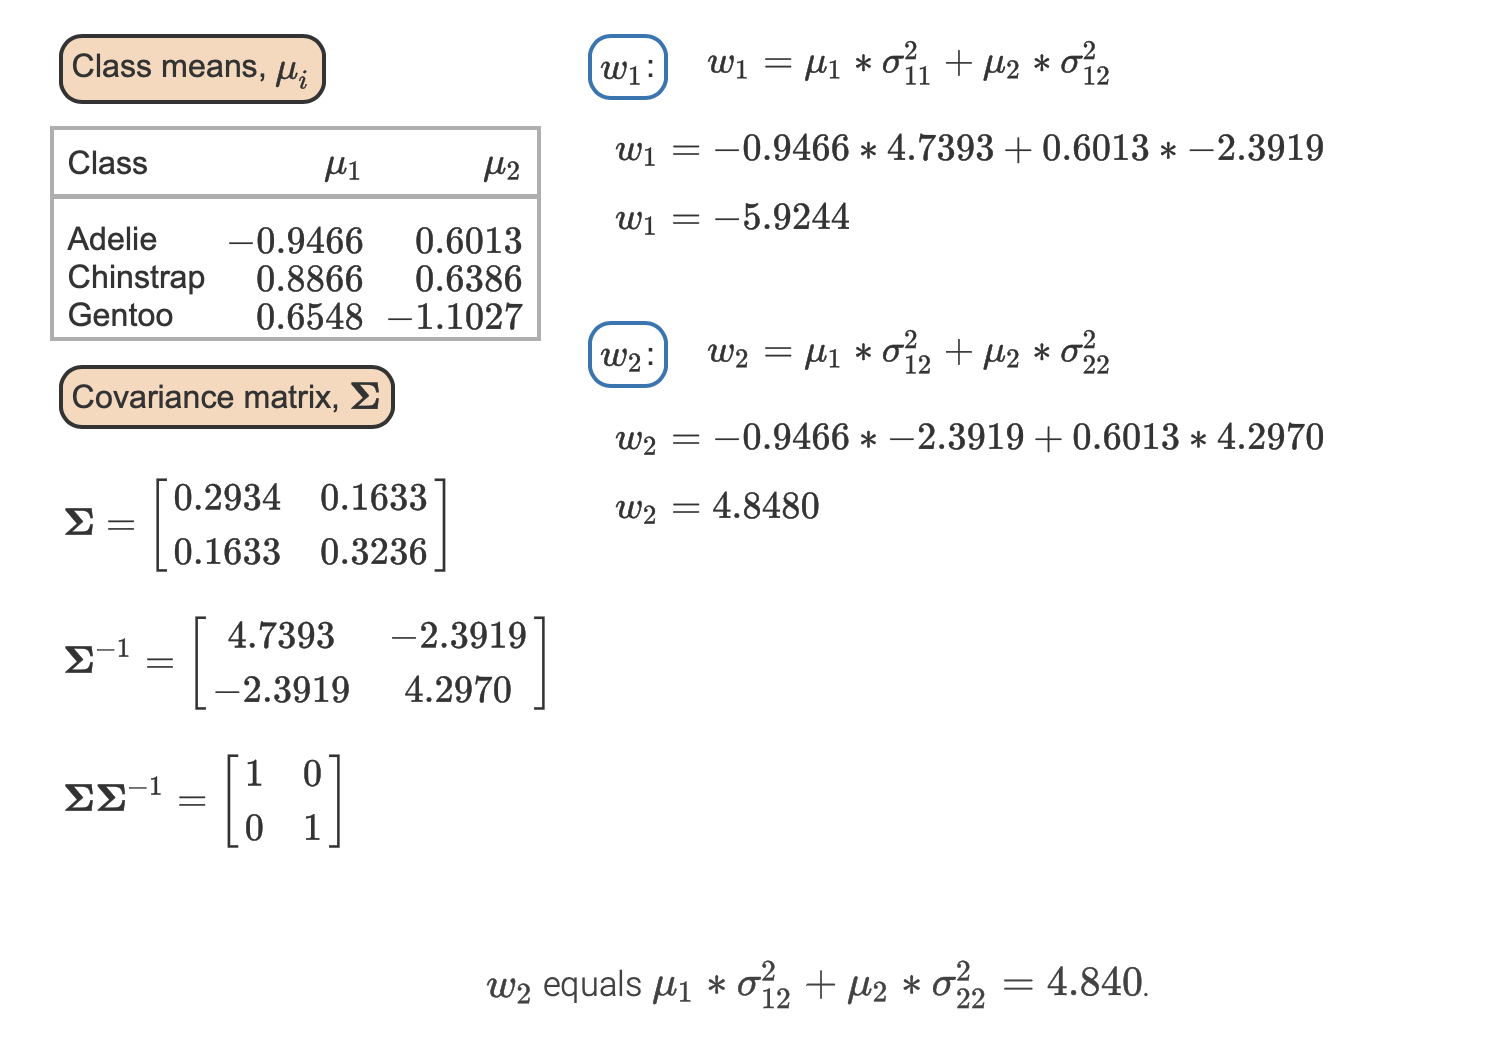
\includegraphics[width=0.8\textwidth]{imgs/df_9.png}
	\end{figure}
\end{frame}

\begin{frame}{Calculating discriminant weights for Adelie penguins.}
	\begin{figure}[ht]
		\centering
		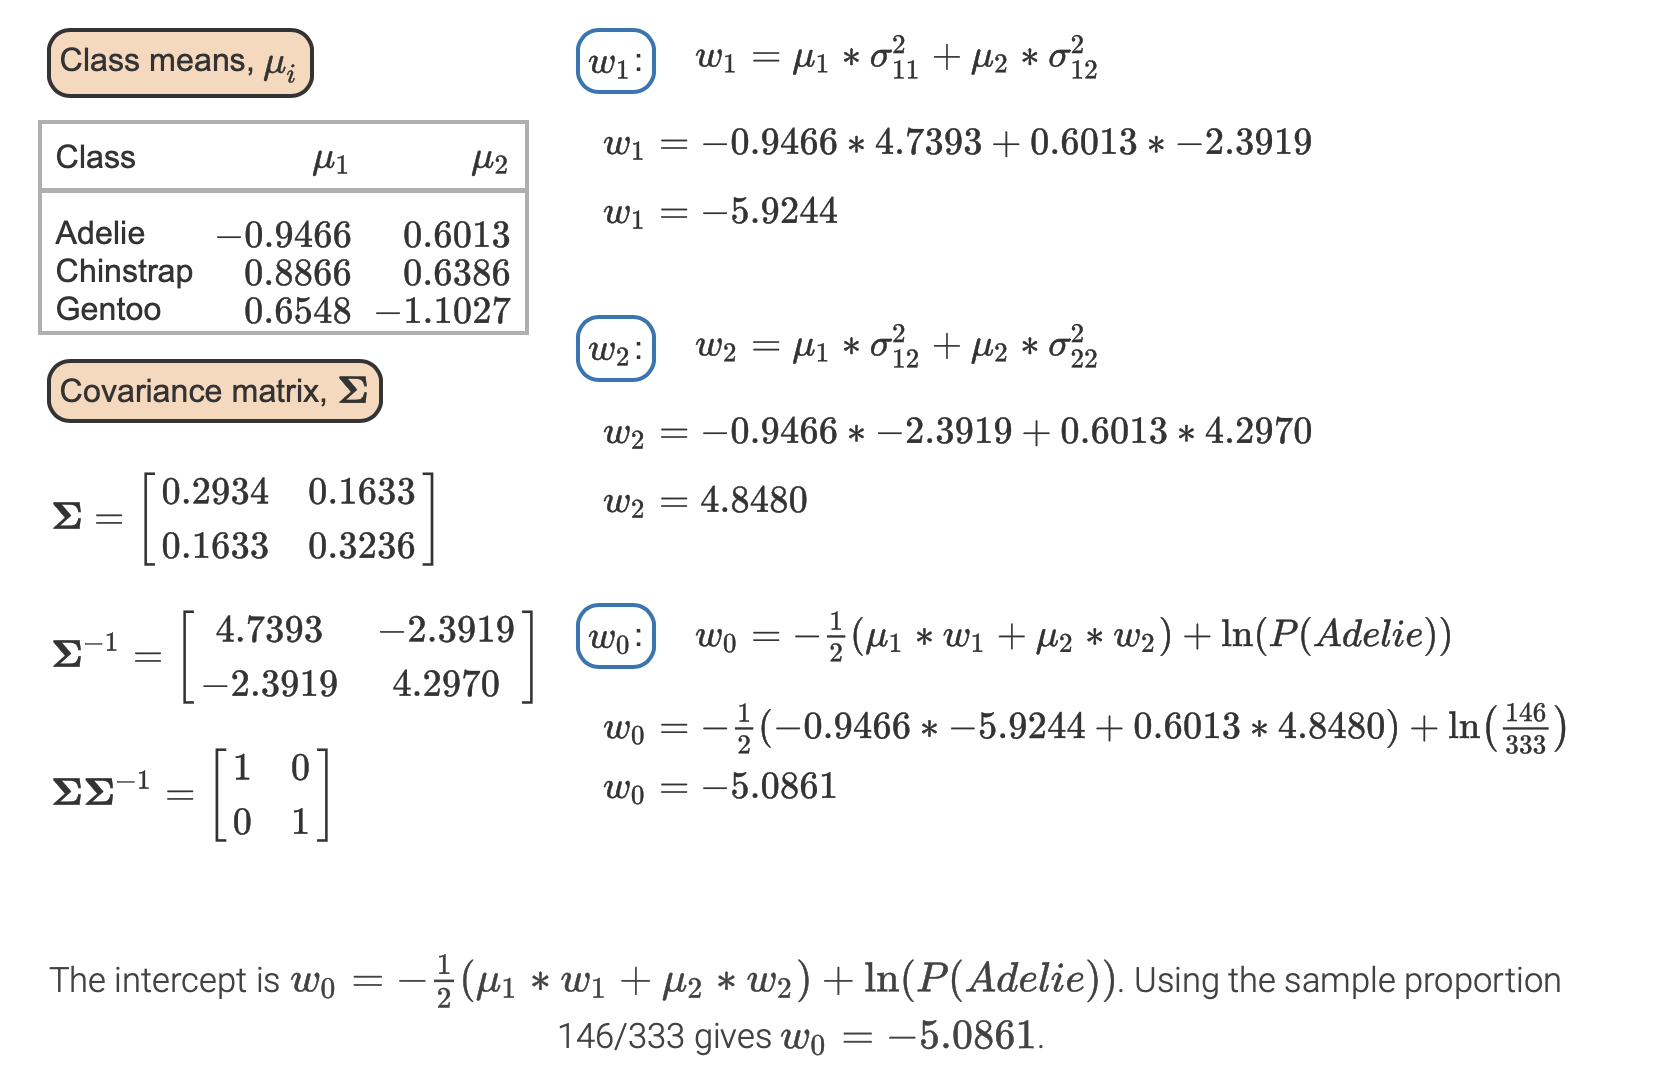
\includegraphics[width=0.8\textwidth]{imgs/df_10.png}
	\end{figure}
\end{frame}

\begin{frame}{Practice Problem: Calculating discriminant weights.}
	\begin{figure}[ht]
		\centering
		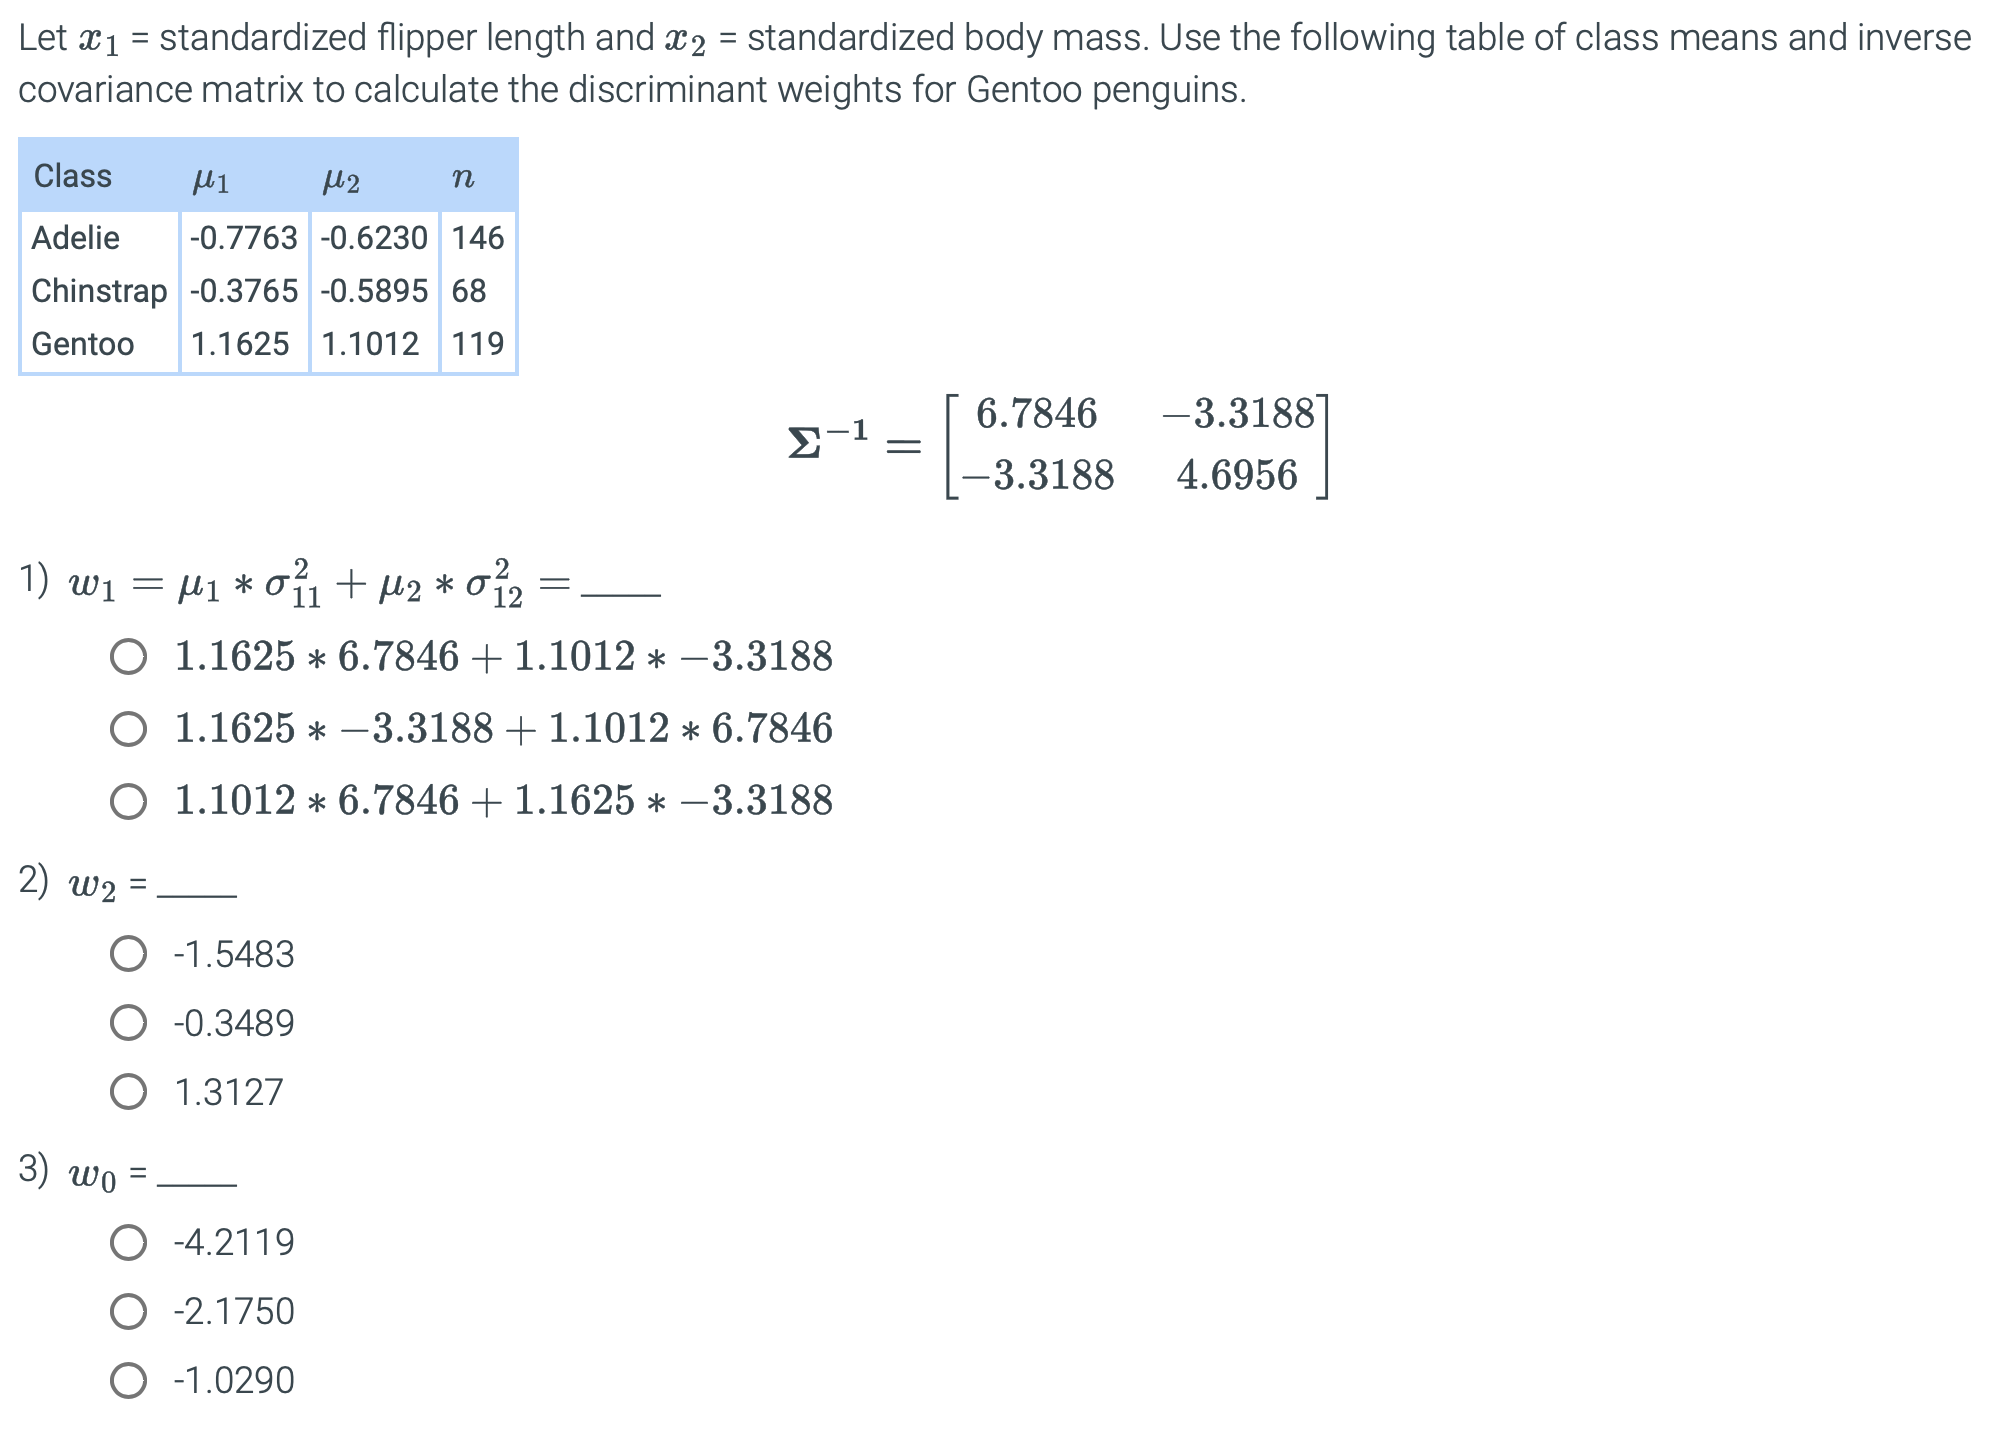
\includegraphics[width=0.8\textwidth]{imgs/df_11.png}
	\end{figure}
\end{frame}

\begin{frame}{Practice Problem: Calculating discriminant weights.}
	\begin{figure}[ht]
		\centering
		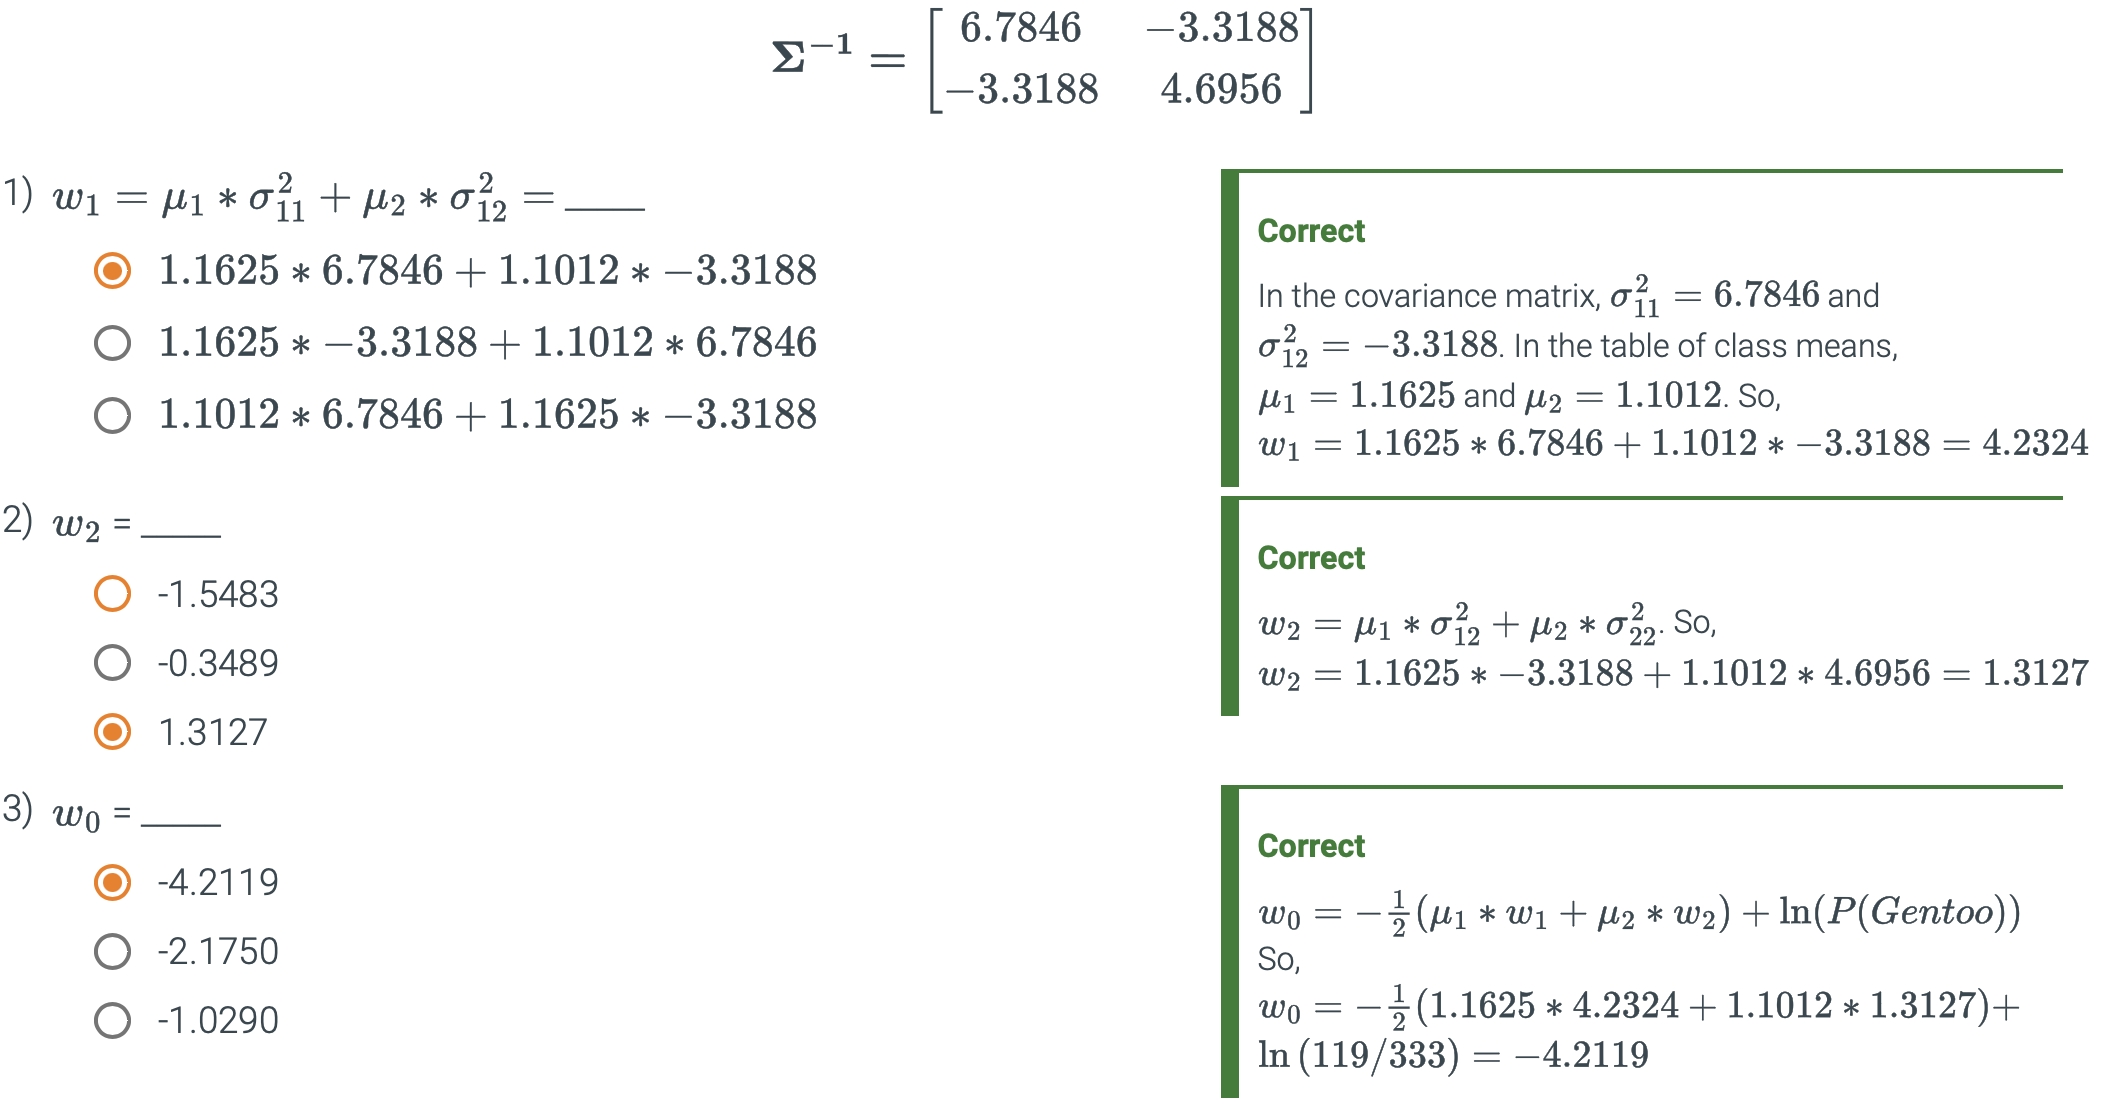
\includegraphics[width=0.8\textwidth]{imgs/df_12.png}
	\end{figure}
\end{frame}

\section{Principal Components}

\begin{frame}{Principal Components}
	Linear discriminant analysis assumes that input features are uncorrelated, which is unrealistic in most cases.
	\begin{itemize}
		\item \textbf{Principal components} is a technique for creating linear combinations of input features that are uncorrelated, called the principal components.
		      In principal components, a set of \(p\) input features is replaced by up to \(p\) linear combinations.
		      $$
			      p c_{j}=\lambda_{1 j} x_{1}+\lambda_{2 j} x_{2}+\ldots+\lambda_{p j} x_{p}
		      $$
	\end{itemize}
\end{frame}

\begin{frame}{Principal Components}
	In principal components, a set of \(p\) input features is replaced by up to \(p\) linear combinations.
	$$
		p c_{j}=\lambda_{1 j} x_{1}+\lambda_{2 j} x_{2}+\ldots+\lambda_{p j} x_{p}
	$$
	\begin{itemize}
		\item The principal component weights, \(\lambda_{i j}\), are chosen such that the resulting principal components \(p c_{i}\) and \(p c_{j}\) are uncorrelated, or
		      independent.
	\end{itemize}
	Since \(p c_{i}\) and \(p c_{j}\) are independent, using principal components satisfies the linear discriminant assumption of uncorrelated
	input features. As a result, linear discriminant functions are often estimated based on the principal components rather than the original
	inputs.
\end{frame}

\begin{frame}
	First thing first, PCA only works for continous variables. With that in mind, let's continue with the examples.

	Given a dataset with 2 features, \(X_1\) and \(X_2\), as follows:

	\[
		\begin{array}{cc}
			\textbf{Feature } X_1 & \textbf{Feature } X_2 \\
			2                     & 1                     \\
			4                     & 3                     \\
			6                     & 5                     \\
			8                     & 7                     \\
		\end{array}
	\]

\end{frame}

\begin{frame}{How do we do PCA?}
	First, \textbf{standardize} each feature to have a mean of 0 and a standard deviation of 1.
	$$
		Z_{i}=\frac{X_{i}-\mu_{i}}{\sigma_{i}}
	$$
	Second, \textbf{compute the covariance matrix} \(\Sigma\) of the standardized features \(Z_{1}\) and \(Z_{2}\) :
	$$
		\Sigma=\frac{1}{n-1} \sum(Z-\bar{Z})(Z-\bar{Z})^{T}
	$$
	Third, do a \textbf{eigendecomposition}, find eigenvalues (\(\lambda\)) and eigenvectors (\(v\)) of \(\Sigma\), and the principal components, are represented by the eigenvectors of covariance matrix:

	\[
		\Sigma v = \lambda v
	\]
\end{frame}

\begin{frame}{Applying Principal Components.}
	\begin{figure}[ht]
		\centering
		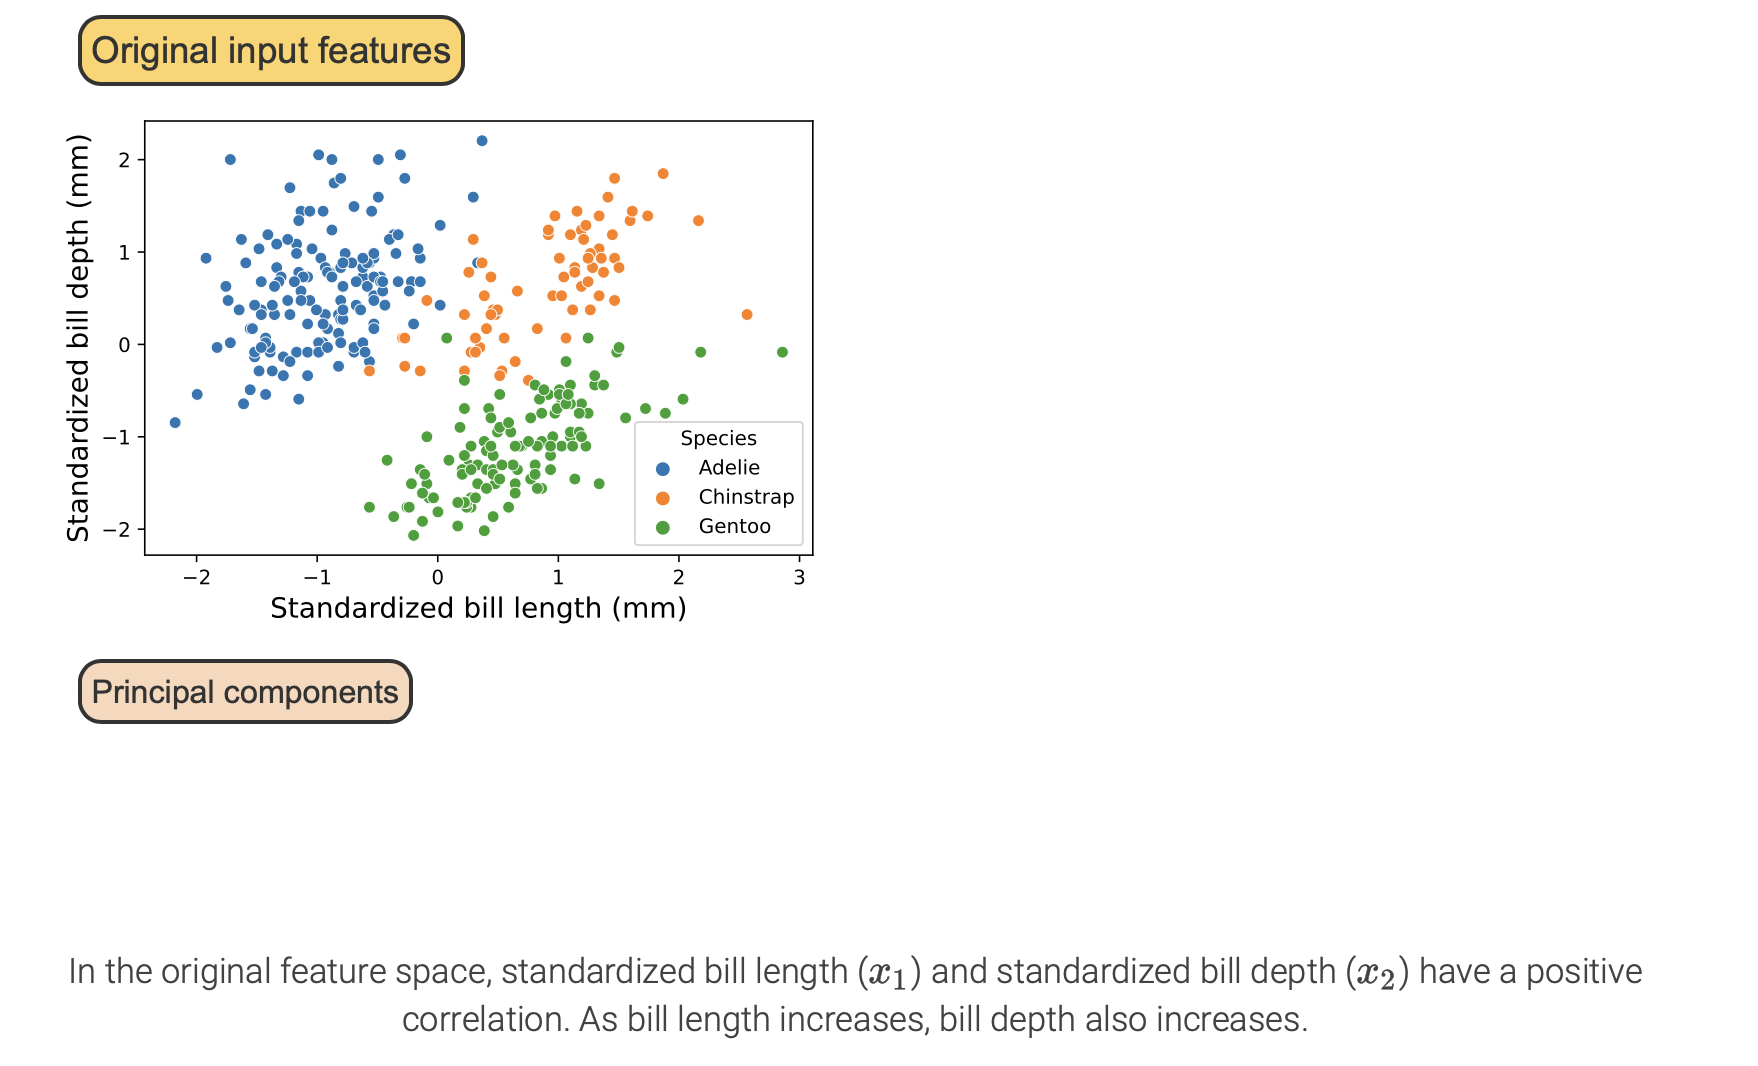
\includegraphics[width=0.8\textwidth]{imgs/df_13.png}
	\end{figure}
\end{frame}

\begin{frame}{Applying Principal Components.}
	\begin{figure}[ht]
		\centering
		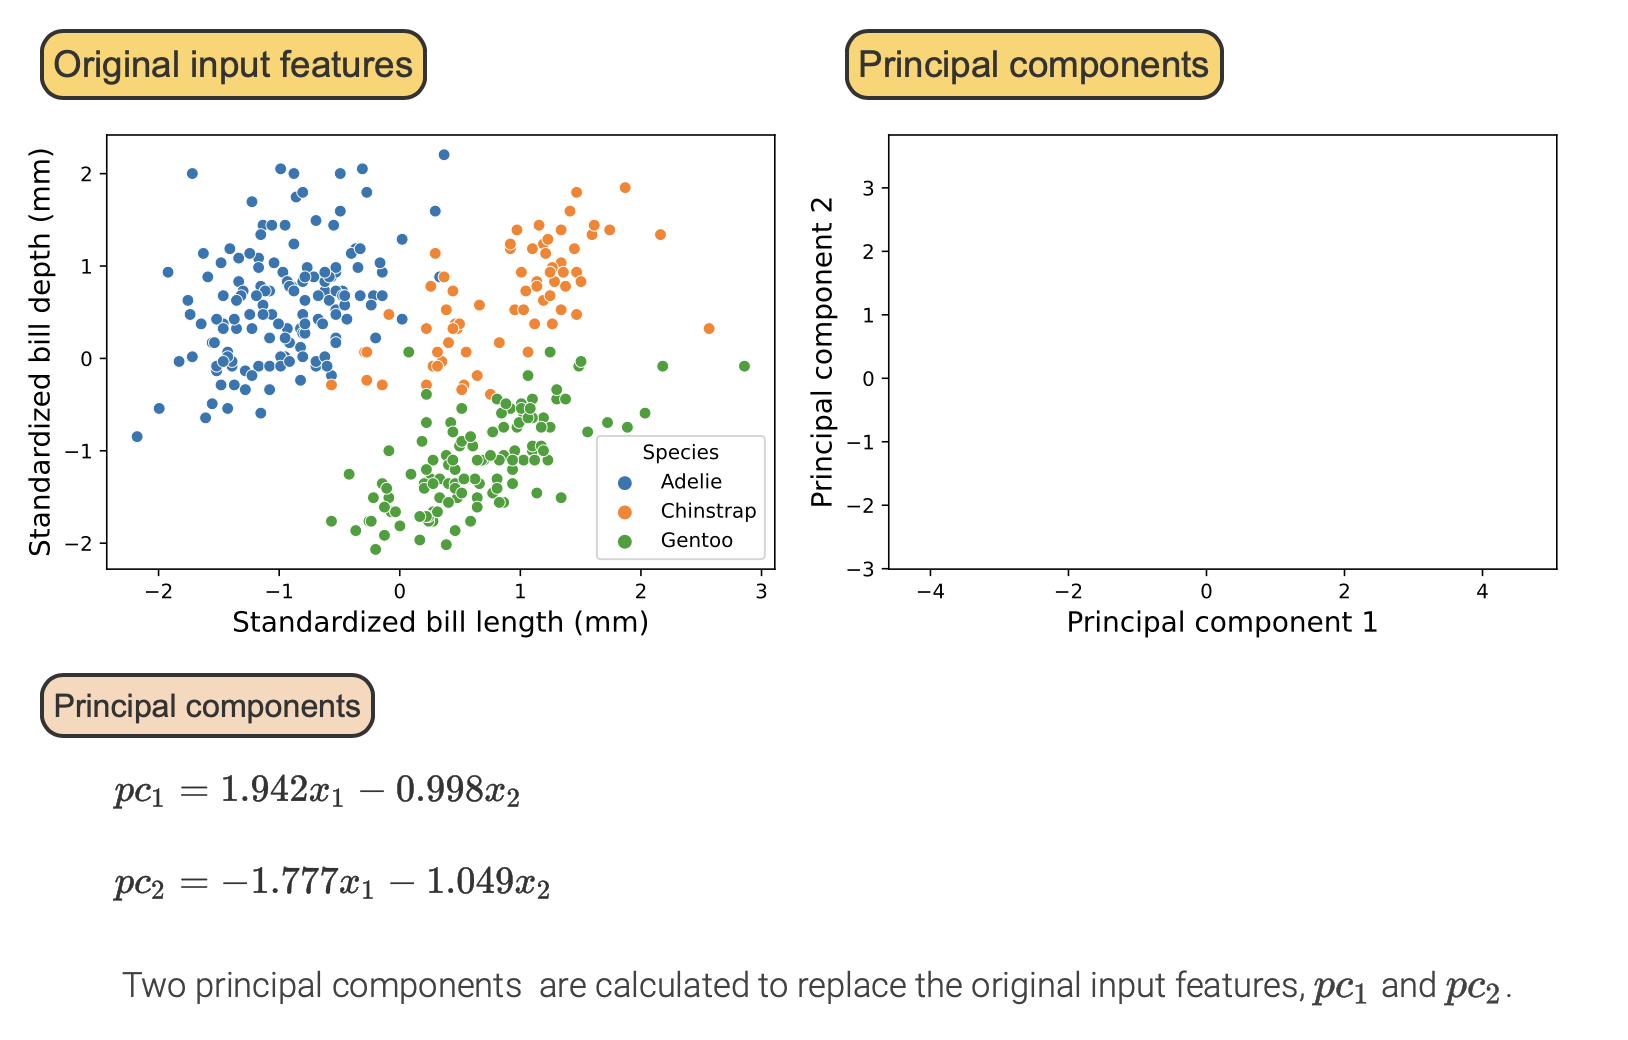
\includegraphics[width=0.8\textwidth]{imgs/df_14.png}
	\end{figure}
\end{frame}

\begin{frame}{Applying Principal Components.}
	\begin{figure}[ht]
		\centering
		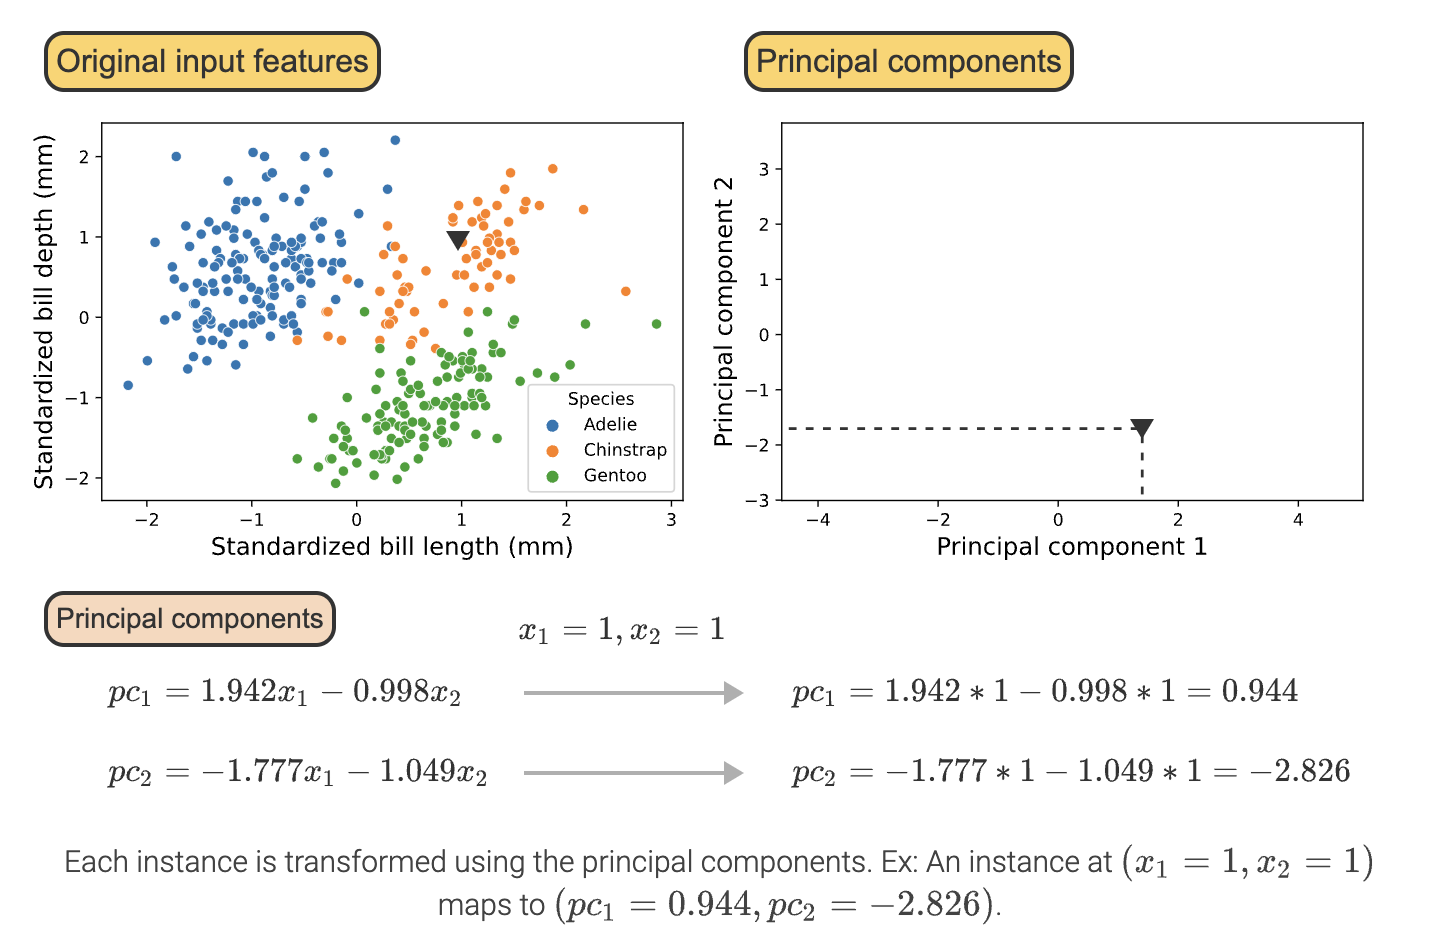
\includegraphics[width=0.8\textwidth]{imgs/df_15.png}
	\end{figure}
\end{frame}

\begin{frame}{Applying Principal Components.}
	\begin{figure}[ht]
		\centering
		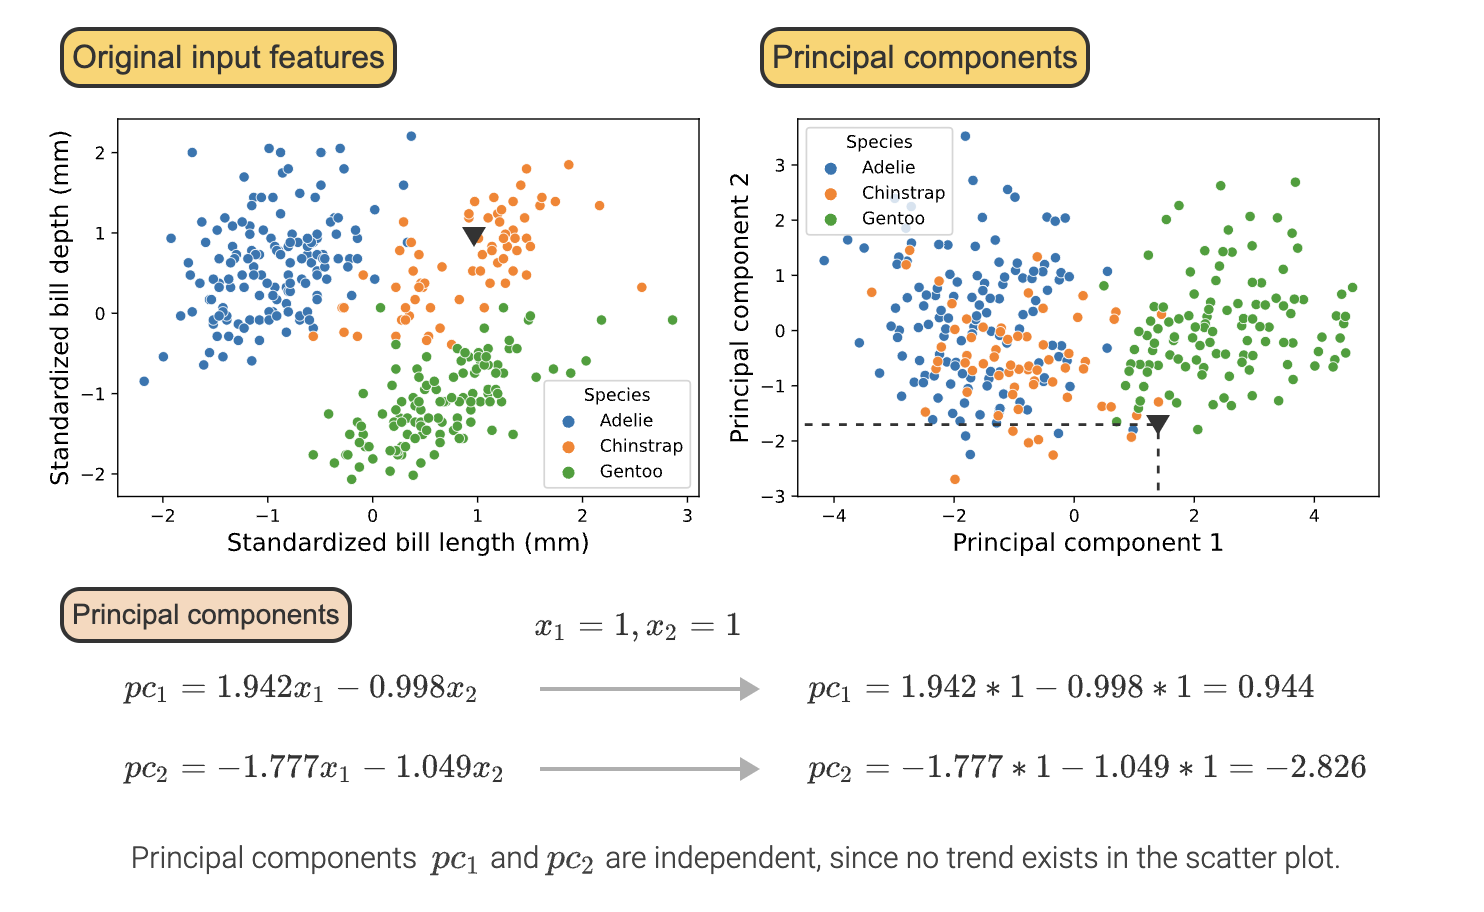
\includegraphics[width=0.8\textwidth]{imgs/df_16.png}
	\end{figure}
\end{frame}

\begin{frame}
	\frametitle{Advantages and Disadvantages}
	Linear discriminant analysis extends to any number of classes, and the prior assumptions about class probabilities can be adjusted to better reflect reality or prior information.
	\begin{itemize}
		\item Ex: A previous study may have measured penguin populations at a different location, which could be incorporated into the prior probabilities. Using principal components as an intermediate step avoids issues with correlated input features. But, restricting the discriminant functions to linear equations results in a linear decision boundary.
	\end{itemize}

	Quadratic discriminant analysis uses quadratic equations in the discriminant functions. The resulting discriminant equations are more complicated, but in some situations a curved decision boundary is a better fit. A tradeoff exists between model complexity and interpretability—models that are more complex are less interpretable.
\end{frame}
\end{document}